%%%%%%%%%%%%%%%%%%%%%%%%%%%%%%%%%%%%%%
\section{Model}
\label{sec:model}
%%%%%%%%%%%%%%%%%%%%%%%%%%%%%%%%%%%%%%

In Lamports original paper on the byzantine generals problem a two algorithms
were proposed, along with impossibility results for reaching
consensus~\cite{Lamport:1982:BGP:357172.357176}. Their theorems proved that
Consensus among generals is impossible, under the condition that generals can
forge messages, if more than one third of the generals is byzantine. Further,
they demonstrate that if messages are sealed with an unforgable signature,
byzantine fault tolerance can be achieved with $n-1$ byzantine generals. Here
we define our model of a distributed system and describe three granularity's of
byzantine fault tolerance. Each granularity is paired with a corresponding
configuration with which use Obeah, and systems which have achieved the
corresponding tolerance.

\subsection{Byzantine Distributed System Model}

We define a distributed system to be composed of $N$ nodes where $N = \{n_1,
n_2, \dots, n_n$\}. Each node can communicate with other nodes on any number of
channels $C$ where $C = \{c_1, c_2, \dots, c_m\}$. Any node may fail, or resume
execution at any time. Channels may drop, reorder, and manipulate messages. We
define the set $B$ where $B \subset N$ to be the number of byzantine nodes in a
system. Byzantine nodes can behave arbitrarily, and antagonistically, with the
possibility to collude with other byzantine nodes in the system.

Nodes instrumented by Obeah are Byzantine to the rest of the nodes in the
system. From the perspective of a node instrumented with Obeah all other nodes,
and all channels in the system are byzantine.


\subsection{Single Byzantine Node}

Many distributed systems dismiss the need to protect against byzantine fault
tolerance. Any admission of byzantine tolerance requires a formalization of the
degree of fault tolerance their system can adhere to. However, all distributed
systems must account for non-determinism in the network, messages can be
reordered or dropped, and correct systems must survive them. Protecting against
a single byzantine node, is similar to protecting against the network, as it
can generate arbitrary messages, and fail to respond, mimicking a partition.

This level of fault tolerance requires a single node in a system, where $N > 3$
to be instrumented with Obeah. Figure~\ref{fig:single-byzantine} visualizes this configuration. We
propose that any implementation of fault tolerant consensus such as
Paxos~\cite{Lamport2001Paxos}, Raft~\cite{184040} or 3PC~\cite{1703048} must
handel these failures.

\begin{figure}[h]
    \centering
    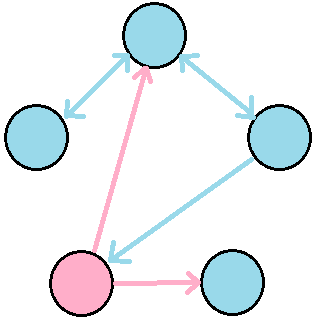
\includegraphics[width=0.5\linewidth]{fig/one-byzantine}%
    \caption{System consisting of a single byzantine node\label{fig:single-byzantine}}%
\end{figure}

\subsection{$N/3 -1$}

Lamports proposed an algorithm for solving the byzantine generals problem in
which $N/3-1$ generals are byzantine. In short the algorithm states that for
any propositions by a general, if all other generals confer with one another on
the proposition they received, consensus among non-byzantine generals can be
reached.

In order to simulate such a scenario $N/3 - 1$ instance of instrumented Obeah
nodes must be run together in a cluster. Figure~\ref{fig:quarum-byzantine}
visualizes this configuration. File systems such as NFS have achieved this
level of fault tolerance with minimal
overhead~\cite{Castro:1999:PBF:296806.296824}.

\begin{figure}[h] 
    \centering
    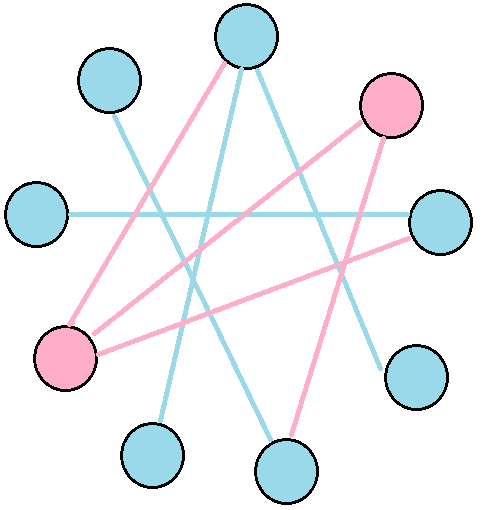
\includegraphics[width=0.5\linewidth]{fig/quarum-byzantine}%
    \caption{System consisting of $N/3 -1$ byzantine nodes\label{fig:quarum-byzantine}}% 
\end{figure}

\subsection{$N-1$}

Finally some systems require the complete resilience of any given node subject all other nodes being byzantine. Lamport proposes by using an unforgable signature on each messages, an recursively passing all received messages to all other nodes, consensus can be reached where $B = N -1$.

To simulate this scenario all but a single node should be executed in an
environment of Obeah instrumented nodes. Figure~\ref{fig:n-1byzantine} visualizes this
configuration. Digital currency systems such a BitCoin have achieved this level
of resilience through the use of iterative public key
encryption~\cite{Nakamoto_bitcoin:a}.

\begin{figure}[h] 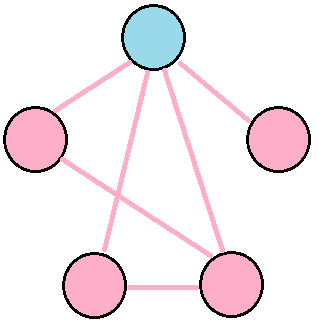
\includegraphics[width=0.5\linewidth]{fig/n-1byzantine}%
    \caption{System consisting of $N-1$ byzantine nodes\label{fig:n-1byzantine}}% 
\end{figure}
